\begin{figure*}
  %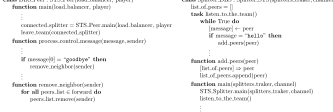
\includegraphics[width=0.55\textwidth]{leaving}
  \fig{300}{4cm}{leaving}
  \caption{Peer leaving.\label{fig:leaving}}
\end{figure*}
An outgoing peer ${\cal P}^j_o$ (see Fig.~\ref{fig:leaving}) from team
${\cal T}_j$ must to: (1) say $[\mathtt{goodbye}]$ to ${\cal S}_j$ and
to ${\cal T}_j$
%$N({\cal P}_o)$
(in this order), (2) relay any pending (received but yet not sent)
chunks, and (3) wait for a $[\mathtt{goodbye}]$ from ${\cal S}_j$,
which performs ${\cal T}_j = {\cal T}_j \setminus {\cal P}^j_o$. In
case of timeout, ${\cal P}^j_o$ resets the leaving procedure, for a
number of times. When a ${\cal P}^j_k\in {\cal T}^k_j$
%${\cal P}_k\in N({\cal P}_i)$
receives a
$[\mathtt{goodbye}]$ from ${\cal P}^j_o$, ${\cal P}^j_k$ removes
%${\cal T}_j = {\cal T}_j \setminus {\cal P}_o$,
${\cal P}^j_o$ from its team, be running ${\cal T}^k_j = {\cal T}^k_j \setminus {\cal P}^j_o$.
%as a neighbor.
%, and finds the
%closest neighbor in ${\cal T}_j \setminus N({\cal X})$ by sending a
%$[\mathtt{hello}]$ to each of them and selecting the closest in terms
%of RTT (see \ref{dbs:joining}).

\begin{comment}
calls the Procedure \emph{Joining a
  team} (for $K=1$), to find a new neighbor. Finally, ${\cal S}_j$
sends to ${\cal P}_o$ a $[\mathtt{goodbye}]$ and performs ${\cal T}_j
= {\cal T}_j \setminus \{{\cal P}_o\}$.
\end{comment}
